\documentclass[10pt,ignorenonframetext,,aspectratio=149]{beamer}
\usefonttheme{serif} % use mainfont rather than sansfont for slide text
\setbeamertemplate{caption}[numbered]
\setbeamertemplate{caption label separator}{: }
\setbeamercolor{caption name}{fg=normal text.fg}
\usepackage{lmodern}
\usepackage{amssymb,amsmath}
\usepackage{ifxetex,ifluatex}
\usepackage{fixltx2e} % provides \textsubscript
\ifnum 0\ifxetex 1\fi\ifluatex 1\fi=0 % if pdftex
  \usepackage[T1]{fontenc}
  \usepackage[utf8]{inputenc}
\else % if luatex or xelatex
  \ifxetex
    \usepackage{mathspec}
  \else
    \usepackage{fontspec}
  \fi
  \defaultfontfeatures{Ligatures=TeX,Scale=MatchLowercase}
  \newcommand{\euro}{€}
    \setmainfont[]{Open Sans}
\fi
% use upquote if available, for straight quotes in verbatim environments
\IfFileExists{upquote.sty}{\usepackage{upquote}}{}
% use microtype if available
\IfFileExists{microtype.sty}{%
\usepackage{microtype}
\UseMicrotypeSet[protrusion]{basicmath} % disable protrusion for tt fonts
}{}
\usepackage{color}
\usepackage{fancyvrb}
\newcommand{\VerbBar}{|}
\newcommand{\VERB}{\Verb[commandchars=\\\{\}]}
\DefineVerbatimEnvironment{Highlighting}{Verbatim}{commandchars=\\\{\}}
% Add ',fontsize=\small' for more characters per line
\usepackage{framed}
\definecolor{shadecolor}{RGB}{248,248,248}
\newenvironment{Shaded}{\begin{snugshade}}{\end{snugshade}}
\newcommand{\AlertTok}[1]{\textcolor[rgb]{0.94,0.16,0.16}{#1}}
\newcommand{\AnnotationTok}[1]{\textcolor[rgb]{0.56,0.35,0.01}{\textbf{\textit{#1}}}}
\newcommand{\AttributeTok}[1]{\textcolor[rgb]{0.77,0.63,0.00}{#1}}
\newcommand{\BaseNTok}[1]{\textcolor[rgb]{0.00,0.00,0.81}{#1}}
\newcommand{\BuiltInTok}[1]{#1}
\newcommand{\CharTok}[1]{\textcolor[rgb]{0.31,0.60,0.02}{#1}}
\newcommand{\CommentTok}[1]{\textcolor[rgb]{0.56,0.35,0.01}{\textit{#1}}}
\newcommand{\CommentVarTok}[1]{\textcolor[rgb]{0.56,0.35,0.01}{\textbf{\textit{#1}}}}
\newcommand{\ConstantTok}[1]{\textcolor[rgb]{0.00,0.00,0.00}{#1}}
\newcommand{\ControlFlowTok}[1]{\textcolor[rgb]{0.13,0.29,0.53}{\textbf{#1}}}
\newcommand{\DataTypeTok}[1]{\textcolor[rgb]{0.13,0.29,0.53}{#1}}
\newcommand{\DecValTok}[1]{\textcolor[rgb]{0.00,0.00,0.81}{#1}}
\newcommand{\DocumentationTok}[1]{\textcolor[rgb]{0.56,0.35,0.01}{\textbf{\textit{#1}}}}
\newcommand{\ErrorTok}[1]{\textcolor[rgb]{0.64,0.00,0.00}{\textbf{#1}}}
\newcommand{\ExtensionTok}[1]{#1}
\newcommand{\FloatTok}[1]{\textcolor[rgb]{0.00,0.00,0.81}{#1}}
\newcommand{\FunctionTok}[1]{\textcolor[rgb]{0.00,0.00,0.00}{#1}}
\newcommand{\ImportTok}[1]{#1}
\newcommand{\InformationTok}[1]{\textcolor[rgb]{0.56,0.35,0.01}{\textbf{\textit{#1}}}}
\newcommand{\KeywordTok}[1]{\textcolor[rgb]{0.13,0.29,0.53}{\textbf{#1}}}
\newcommand{\NormalTok}[1]{#1}
\newcommand{\OperatorTok}[1]{\textcolor[rgb]{0.81,0.36,0.00}{\textbf{#1}}}
\newcommand{\OtherTok}[1]{\textcolor[rgb]{0.56,0.35,0.01}{#1}}
\newcommand{\PreprocessorTok}[1]{\textcolor[rgb]{0.56,0.35,0.01}{\textit{#1}}}
\newcommand{\RegionMarkerTok}[1]{#1}
\newcommand{\SpecialCharTok}[1]{\textcolor[rgb]{0.00,0.00,0.00}{#1}}
\newcommand{\SpecialStringTok}[1]{\textcolor[rgb]{0.31,0.60,0.02}{#1}}
\newcommand{\StringTok}[1]{\textcolor[rgb]{0.31,0.60,0.02}{#1}}
\newcommand{\VariableTok}[1]{\textcolor[rgb]{0.00,0.00,0.00}{#1}}
\newcommand{\VerbatimStringTok}[1]{\textcolor[rgb]{0.31,0.60,0.02}{#1}}
\newcommand{\WarningTok}[1]{\textcolor[rgb]{0.56,0.35,0.01}{\textbf{\textit{#1}}}}
\usepackage{graphicx,grffile}
\makeatletter
\def\maxwidth{\ifdim\Gin@nat@width>\linewidth\linewidth\else\Gin@nat@width\fi}
\def\maxheight{\ifdim\Gin@nat@height>\textheight0.8\textheight\else\Gin@nat@height\fi}
\makeatother
% Scale images if necessary, so that they will not overflow the page
% margins by default, and it is still possible to overwrite the defaults
% using explicit options in \includegraphics[width, height, ...]{}
\setkeys{Gin}{width=\maxwidth,height=\maxheight,keepaspectratio}

% Comment these out if you don't want a slide with just the
% part/section/subsection/subsubsection title:
\AtBeginPart{
  \let\insertpartnumber\relax
  \let\partname\relax
  \frame{\partpage}
}
\AtBeginSection{
  \let\insertsectionnumber\relax
  \let\sectionname\relax
  \frame{\sectionpage}
}
\AtBeginSubsection{
  \let\insertsubsectionnumber\relax
  \let\subsectionname\relax
  \frame{\subsectionpage}
}

\setlength{\emergencystretch}{3em}  % prevent overfull lines
\providecommand{\tightlist}{%
  \setlength{\itemsep}{0pt}\setlength{\parskip}{0pt}}
\setcounter{secnumdepth}{0}

\title{SNA, Centrality dan Modularity}
\subtitle{(Pelatihan data sains menggunakan R dan Gephi)}
\author{Ujang Fahmi}
\date{}

%% Here's everything I added.
%%--------------------------

\usepackage{graphicx}
\usepackage{rotating}
%\setbeamertemplate{caption}[numbered]
\usepackage{hyperref}
\usepackage{caption}
\usepackage[normalem]{ulem}
%\mode<presentation>
\usepackage{wasysym}
%\usepackage{amsmath}


% Get rid of navigation symbols.
%-------------------------------
\setbeamertemplate{navigation symbols}{}

% Optional institute tags and titlegraphic.
% Do feel free to change the titlegraphic if you don't want it as a Markdown field.
%----------------------------------------------------------------------------------
\institute{Pelajaran ke-09}

% \titlegraphic{\includegraphics[width=0.3\paperwidth]{\string~/Dropbox/teaching/clemson-academic.png}} % <-- if you want to know what this looks like without it as a Markdown field. 
% -----------------------------------------------------------------------------------------------------
\titlegraphic{
\includegraphics[width=0.3\paperwidth]{styles/sadasa.png}}

% Some additional title page adjustments.
%----------------------------------------
\setbeamertemplate{title page}[empty]
%\date{}
\setbeamerfont{subtitle}{size=\small}

\setbeamercovered{transparent}

% Some optional colors. Change or add as you see fit.
%---------------------------------------------------
\definecolor{clemsonpurple}{HTML}{522D80}
 \definecolor{clemsonorange}{HTML}{F66733}
\definecolor{uiucblue}{HTML}{003C7D}
\definecolor{uiucorange}{HTML}{F47F24}


% Some optional color adjustments to Beamer. Change as you see fit.
%------------------------------------------------------------------
\setbeamercolor{frametitle}{fg=clemsonpurple,bg=white}
\setbeamercolor{title}{fg=clemsonpurple,bg=white}
\setbeamercolor{local structure}{fg=clemsonpurple}
\setbeamercolor{section in toc}{fg=clemsonpurple,bg=white}
% \setbeamercolor{subsection in toc}{fg=clemsonorange,bg=white}
\setbeamercolor{footline}{fg=clemsonpurple!50, bg=white}
\setbeamercolor{block title}{fg=clemsonorange,bg=white}


\let\Tiny=\tiny


% Sections and subsections should not get their own damn slide.
%--------------------------------------------------------------
\AtBeginPart{}
\AtBeginSection{}
\AtBeginSubsection{}
\AtBeginSubsubsection{}

% Suppress some of Markdown's weird default vertical spacing.
%------------------------------------------------------------
\setlength{\emergencystretch}{0em}  % prevent overfull lines
\setlength{\parskip}{0pt}


% Allow for those simple two-tone footlines I like. 
% Edit the colors as you see fit.
%--------------------------------------------------
\defbeamertemplate*{footline}{my footline}{%
    \ifnum\insertpagenumber=1
    \hbox{%
        \begin{beamercolorbox}[wd=\paperwidth,ht=.8ex,dp=1ex,center]{}%
      % empty environment to raise height
        \end{beamercolorbox}%
    }%
    \vskip0pt%
    \else%
        \Tiny{%
            \hfill%
		\vspace*{1pt}%
            \insertframenumber/\inserttotalframenumber \hspace*{0.1cm}%
            \newline%
            \color{clemsonpurple}{\rule{\paperwidth}{0.4mm}}\newline%
            \color{clemsonorange}{\rule{\paperwidth}{.4mm}}%
        }%
    \fi%
}

% Various cosmetic things, though I must confess I forget what exactly these do and why I included them.
%-------------------------------------------------------------------------------------------------------
\setbeamercolor{structure}{fg=blue}
\setbeamercolor{local structure}{parent=structure}
\setbeamercolor{item projected}{parent=item,use=item,fg=clemsonpurple,bg=white}
\setbeamercolor{enumerate item}{parent=item}

% Adjust some item elements. More cosmetic things.
%-------------------------------------------------
\setbeamertemplate{itemize item}{\color{clemsonpurple}$\bullet$}
\setbeamertemplate{itemize subitem}{\color{clemsonpurple}\scriptsize{$\bullet$}}
\setbeamertemplate{itemize/enumerate body end}{\vspace{.6\baselineskip}} % So I'm less inclined to use \medskip and \bigskip in Markdown.

% Automatically center images
% ---------------------------
% Note: this is for ![](image.png) images
% Use "fig.align = "center" for R chunks

\usepackage{etoolbox}

\AtBeginDocument{%
  \letcs\oig{@orig\string\includegraphics}%
  \renewcommand<>\includegraphics[2][]{%
    \only#3{%
      {\centering\oig[{#1}]{#2}\par}%
    }%
  }%
}

% I think I've moved to xelatex now. Here's some stuff for that.
% --------------------------------------------------------------
% I could customize/generalize this more but the truth is it works for my circumstances.

\ifxetex
\setbeamerfont{title}{family=\fontspec{Titillium Web}}
\setbeamerfont{frametitle}{family=\fontspec{Titillium Web}}
\usepackage[font=small,skip=0pt]{caption}
 \else
 \fi

% Okay, and begin the actual document...

\begin{document}
\frame{\titlepage}

\begin{frame}
Salam kenal dan selamat datang.

Semoga kita semua bisa saling berbagi pengalaman dan pengetahuan. Saya
adalah Ujang Fahmi, Co-founder dan mentor Sadasa Academy.

\vspace{0.1in}

Jika anda berada dan sedang membaca tutorial ini, maka kemungkinan anda
adalah orang yang sedang ingin belajar data sains, atau mungkin
ditugaskan untuk mempelajari R oleh institusi atau organisasi anda. Sama
seperti saya dulu, dimana tanpa latar belakang enginering saya
didiharuskan untuk belajar R, demi menyelesaikan tugas akhir dan
akhirnya jadilah seperti saya sekarang ini.

\vspace{0.1in}

Satu hal yang pasti, ini adalah langkah pertama dari banyak langkah yang
harus dilalui, entah melalui lembaga resmi atau belajar secara mandiri.
Jadi selamat belajar!!!

\vspace{0.1in}

Ujang Fahmi,

Yogyakarta, 2021-09-29

\vspace{0.1in}

\emph{Materi yang disampaikan disimpan dan dokumentasikan}
\href{https://github.com/eppofahmi/belajaR/tree/master/upn-surabaya}{\textbf{disini}}
\end{frame}

\hypertarget{parameter-pengkuran-dalam-sna}{%
\section{Parameter pengkuran dalam
SNA}\label{parameter-pengkuran-dalam-sna}}

\begin{frame}{Parameter pengkuran dalam SNA}
\begin{enumerate}
\item
  Social network analysis (SNA) atau analisis jejaring sosial merupakan
  salah satu metode yang saat ini sering dibicarakan dan banyak
  diaplikasikan untuk berbagai kasus/studi.
\item
  SNA banyak digunakan karena bisa diaplikasikan pada berbagai skenario
  jariangan baik yang melibatkan aktor manusia/username atau aktor bukan
  manusia seperti stasiun/jabatan.
\item
  Mudahnya mendapatkan data, khususnya dari media sosial untuk dijadikan
  sebagai studi.
\end{enumerate}
\end{frame}

\hypertarget{centrality}{%
\subsection{Centrality}\label{centrality}}

\begin{frame}{Centrality}
\begin{columns}[T]
\begin{column}{0.5\textwidth}
Social network analysis is the process of investigating social
structures through the use of networks and graph theory. It
characterizes networked structures in terms of nodes and the ties,
edges, or links that connect them. \vspace{0.1in} Dalam sebuah network
centrality merupakan indikator yang melekat pada sebuah nodes.
Centrality bisa memberikan informasi seperti nodes populer, nodes mana
yang menjadi penghubung, dan nodes yang bisa memengaruhi network dengan
cepat.
\end{column}

\begin{column}{0.5\textwidth}
\begin{figure}
\centering
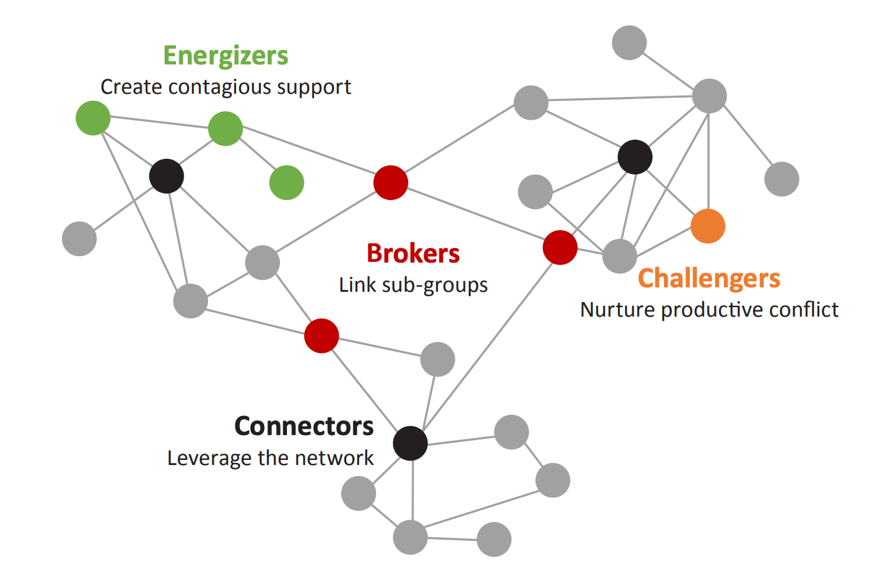
\includegraphics{images/sna1.png}
\caption{Ilustrasi SNA}
\end{figure}
\end{column}
\end{columns}
\end{frame}

\begin{frame}{Degree Centrality}
\protect\hypertarget{degree-centrality}{}
\textbf{Definition}: Degree centrality assigns an importance score based
simply on the number of links held by each node.

\textbf{What it tells us}: How many direct, `one hop' connections each
node has to other nodes in the network.

\textbf{When to use it}: For finding very connected individuals, popular
individuals, individuals who are likely to hold most information or
individuals who can quickly connect with the wider network.

\textbf{A bit more detail}: Degree centrality is the simplest measure of
node connectivity. Sometimes it's useful to look at in-degree (number of
inbound links) and out-degree (number of outbound links) as distinct
measures, for example when looking at transactional data or account
activity.A bit more detail: Degree centrality is the simplest measure of
node connectivity. Sometimes it's useful to look at in-degree (number of
inbound links) and out-degree (number of outbound links) as distinct
measures, for example when looking at transactional data or account
activity.
\end{frame}

\begin{frame}{Betweeness Centrality}
\protect\hypertarget{betweeness-centrality}{}
\textbf{Definition}: Betweenness centrality measures the number of times
a node lies on the shortest path between other nodes.

\textbf{What it tells us}: This measure shows which nodes are `bridges'
between nodes in a network. It does this by identifying all the shortest
paths and then counting how many times each node falls on one.

\textbf{When to use it}: For finding the individuals who influence the
flow around a system.

\textbf{A bit more detail}: Betweenness is useful for analyzing
communication dynamics, but should be used with care. A high betweenness
count could indicate someone holds authority over disparate clusters in
a network, or just that they are on the periphery of both clusters.
\end{frame}

\begin{frame}{Closeness Centrality}
\protect\hypertarget{closeness-centrality}{}
\textbf{Definition}: Closeness centrality scores each node based on
their `closeness' to all other nodes in the network.

\textbf{What it tells us}: This measure calculates the shortest paths
between all nodes, then assigns each node a score based on its sum of
shortest paths.

\textbf{When to use it}: For finding the individuals who are best placed
to influence the entire network most quickly.

\textbf{A bit more detail}: Closeness centrality can help find good
`broadcasters', but in a highly-connected network, you will often find
all nodes have a similar score. What may be more useful is using
Closeness to find influencers in a single cluster.
\end{frame}

\begin{frame}{Eigenvector Centrality}
\protect\hypertarget{eigenvector-centrality}{}
\textbf{Definition}: Like degree centrality, EigenCentrality measures a
node's influence based on the number of links it has to other nodes in
the network. EigenCentrality then goes a step further by also taking
into account how well connected a node is, and how many links their
connections have, and so on through the network.

\textbf{What it tells us}: By calculating the extended connections of a
node, EigenCentrality can identify nodes with influence over the whole
network, not just those directly connected to it.

\textbf{When to use it}: EigenCentrality is a good `all-round' SNA
score, handy for understanding human social networks, but also for
understanding networks like malware propagation.

\textbf{A bit more detail}: Our tools calculate each node's
EigenCentrality by converging on an eigenvector using the power
iteration method.
\end{frame}

\begin{frame}{Page Rank}
\protect\hypertarget{page-rank}{}
\textbf{Definition}: PageRank is a variant of EigenCentrality, also
assigning nodes a score based on their connections, and their
connections' connections. The difference is that PageRank also takes
link direction and weight into account -- so links can only pass
influence in one direction, and pass different amounts of influence.

\textbf{What it tells us}: This measure uncovers nodes whose influence
extends beyond their direct connections into the wider network.

\textbf{When to use it}: Because it takes into account direction and
connection weight, PageRank can be helpful for understanding citations
and authority.

\textbf{A bit more detail}: PageRank is famously one of the ranking
algorithms behind the original Google search engine (the `Page' part of
its name comes from creator and Google founder, Sergei Brin).
\end{frame}

\hypertarget{modularity}{%
\subsection{Modularity}\label{modularity}}

\begin{frame}{Modularity}
\begin{columns}[T]
\begin{column}{0.5\textwidth}
\textbf{Modularity} adalah sebuah perhitungan yang mengukur
kekuatan/kedekatan antar divisi dalam sebuah jejaring dan
mengelompokannya menjadi modul (grup, kluster, atau komunitas).

\vspace{0.1in}

Network yang memiliki moudularity tinggi memiliki densitas koneksi antar
nodes di dalamnya, namun jauh/jarang dengan nodes dari modul/grup lain.
Modularity sering digunakan sebagai metode optimasi untuk mendeteksi
struktur komunitas dalam sebuah jejaring.
\end{column}

\begin{column}{0.5\textwidth}
\begin{figure}
\centering
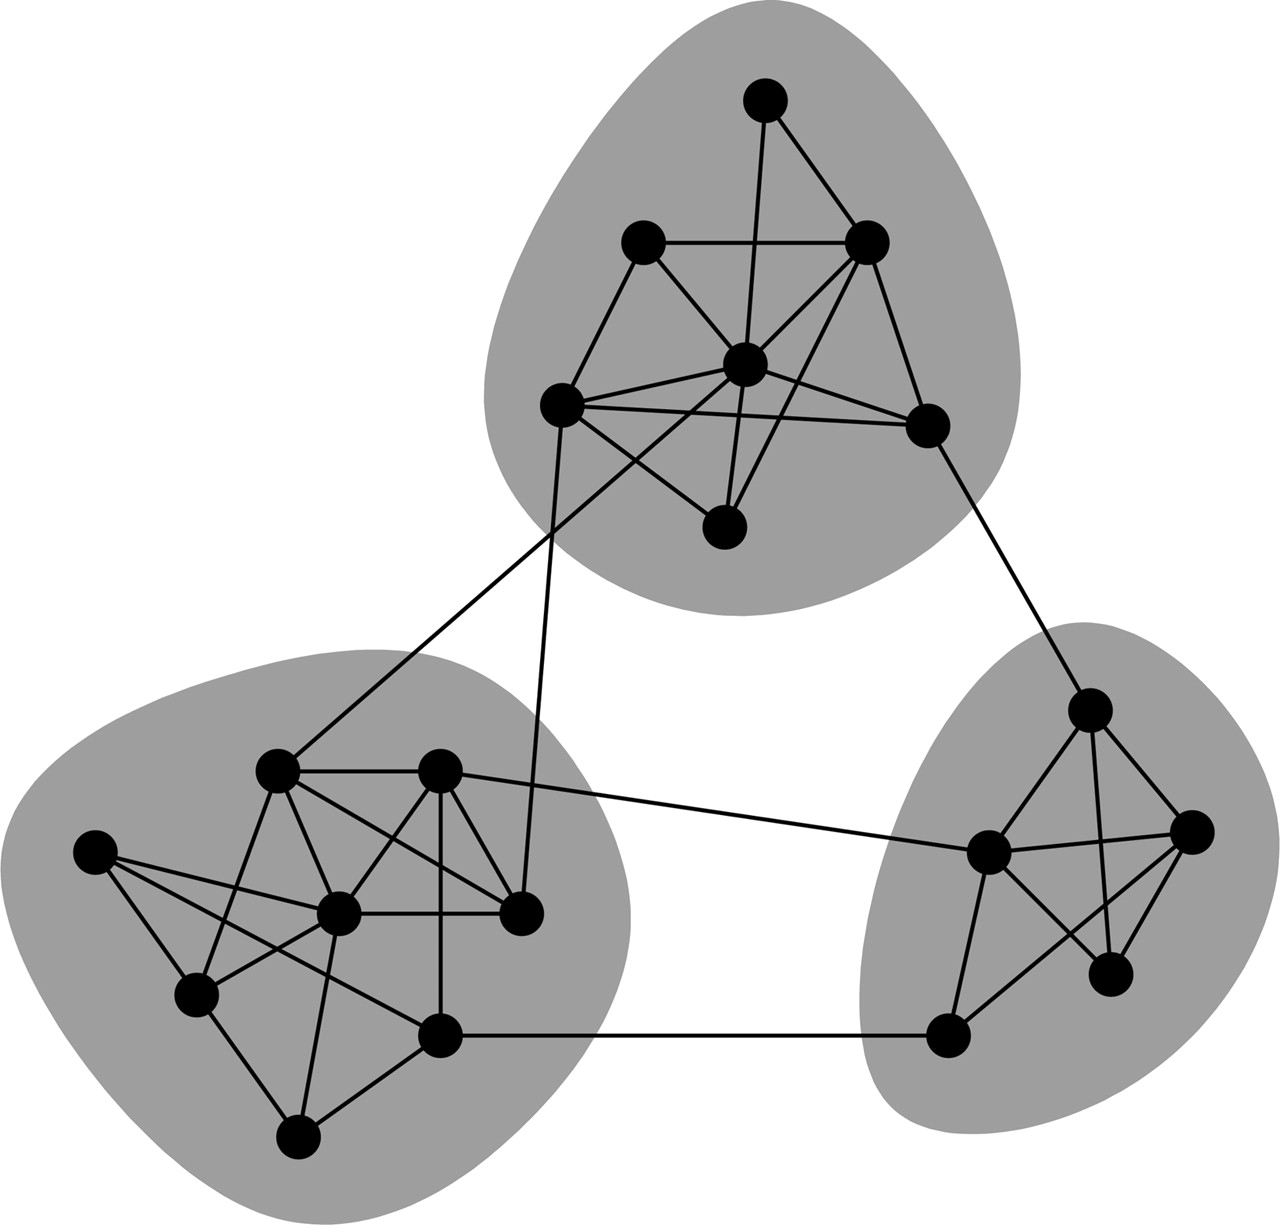
\includegraphics{images/modularity.jpg}
\caption{Ilustrasi Modularity}
\end{figure}
\end{column}
\end{columns}
\end{frame}

\hypertarget{mendapatkan-network-centrality}{%
\section{Mendapatkan Network
Centrality}\label{mendapatkan-network-centrality}}

\hypertarget{degree-centrality-1}{%
\subsection{Degree Centrality}\label{degree-centrality-1}}

\begin{frame}[fragile]{Degree Centrality}
\begin{columns}[T]
\begin{column}{0.5\textwidth}
Degree merupakan struktur paling dasar dalam sebuah jejaring. Degree
bisa didapat dari sebuah graph di r menggunakan fungsi \texttt{degree()}
dari \texttt{igraph}.
\end{column}

\begin{column}{0.5\textwidth}
\begin{Shaded}
\begin{Highlighting}[]
\FunctionTok{library}\NormalTok{(igraph)}

\NormalTok{g }\OtherTok{\textless{}{-}} \FunctionTok{make\_ring}\NormalTok{(}\DecValTok{10}\NormalTok{)}
\FunctionTok{degree}\NormalTok{(g)}
\NormalTok{g2 }\OtherTok{\textless{}{-}} \FunctionTok{sample\_gnp}\NormalTok{(}\DecValTok{1000}\NormalTok{, }\DecValTok{10}\SpecialCharTok{/}\DecValTok{1000}\NormalTok{)}
\FunctionTok{degree\_distribution}\NormalTok{(g2)}
\end{Highlighting}
\end{Shaded}
\end{column}
\end{columns}
\end{frame}

\hypertarget{betweeness-centrality-1}{%
\subsection{Betweeness Centrality}\label{betweeness-centrality-1}}

\begin{frame}[fragile]{Betweeness Centrality}
\begin{columns}[T]
\begin{column}{0.5\textwidth}
Betweeness bisa diterapkan untuk nodes dan edeges. Di igraph kita bisa
menggunakan fungsi \texttt{betweenness()} untuk nodes, dan
\texttt{edge\_betweenness()} untuk edges.
\end{column}

\begin{column}{0.5\textwidth}
\begin{Shaded}
\begin{Highlighting}[]
\FunctionTok{library}\NormalTok{(igraph)}
\NormalTok{g }\OtherTok{\textless{}{-}} \FunctionTok{sample\_gnp}\NormalTok{(}\DecValTok{10}\NormalTok{, }\DecValTok{3}\SpecialCharTok{/}\DecValTok{10}\NormalTok{)}
\FunctionTok{betweenness}\NormalTok{(g)}
\FunctionTok{edge\_betweenness}\NormalTok{(g)}
\end{Highlighting}
\end{Shaded}
\end{column}
\end{columns}
\end{frame}

\hypertarget{closeness-centrality-1}{%
\subsection{Closeness Centrality}\label{closeness-centrality-1}}

\begin{frame}[fragile]{Closeness Centrality}
\begin{columns}[T]
\begin{column}{0.5\textwidth}
Closeness dari sebuah network bisa didapat menggunakan fungsi
\texttt{closeness()} dari \texttt{igraph}. Di sini closeness memiliki
tiga mode dengan mempertimbangkan tipe networknya (directed atau
undirected).
\end{column}

\begin{column}{0.5\textwidth}
\begin{Shaded}
\begin{Highlighting}[]
\NormalTok{g }\OtherTok{\textless{}{-}} \FunctionTok{make\_ring}\NormalTok{(}\DecValTok{10}\NormalTok{)}
\NormalTok{g2 }\OtherTok{\textless{}{-}} \FunctionTok{make\_star}\NormalTok{(}\DecValTok{10}\NormalTok{)}
\FunctionTok{closeness}\NormalTok{(g)}
\FunctionTok{closeness}\NormalTok{(g2, }\AttributeTok{mode=}\StringTok{"in"}\NormalTok{)}
\FunctionTok{closeness}\NormalTok{(g2, }\AttributeTok{mode=}\StringTok{"out"}\NormalTok{)}
\FunctionTok{closeness}\NormalTok{(g2, }\AttributeTok{mode=}\StringTok{"all"}\NormalTok{)}
\end{Highlighting}
\end{Shaded}
\end{column}
\end{columns}
\end{frame}

\hypertarget{eigenvector-centrality-1}{%
\subsection{Eigenvector Centrality}\label{eigenvector-centrality-1}}

\begin{frame}[fragile]{Eigenvector Centrality}
Eigenvector bisa didapatkan dari sebuah graph menggunakan fungsi
\texttt{eigen\_centrality()}.

\begin{Shaded}
\begin{Highlighting}[]
\CommentTok{\#Generate some test data}
\NormalTok{g }\OtherTok{\textless{}{-}} \FunctionTok{make\_ring}\NormalTok{(}\DecValTok{10}\NormalTok{, }\AttributeTok{directed=}\ConstantTok{FALSE}\NormalTok{)}
\CommentTok{\#Compute eigenvector centrality scores}
\FunctionTok{eigen\_centrality}\NormalTok{(g)}
\end{Highlighting}
\end{Shaded}
\end{frame}

\hypertarget{page-rank-1}{%
\subsection{Page Rank}\label{page-rank-1}}

\begin{frame}[fragile]{Page Rank}
Fungsi \texttt{page\_rank()} bisa digunakan untuk mengukur
\texttt{page\_rank()} yaitu sebuah algoritme yang dibuat dan digunakan
oleh google untuk memberikan peringkat pada sebuah laman.

\begin{Shaded}
\begin{Highlighting}[]
\NormalTok{g }\OtherTok{\textless{}{-}} \FunctionTok{sample\_gnp}\NormalTok{(}\DecValTok{20}\NormalTok{, }\DecValTok{5}\SpecialCharTok{/}\DecValTok{20}\NormalTok{, }\AttributeTok{directed=}\ConstantTok{TRUE}\NormalTok{)}
\FunctionTok{page\_rank}\NormalTok{(g)}\SpecialCharTok{$}\NormalTok{vector}

\NormalTok{g2 }\OtherTok{\textless{}{-}} \FunctionTok{make\_star}\NormalTok{(}\DecValTok{10}\NormalTok{)}
\FunctionTok{page\_rank}\NormalTok{(g2)}\SpecialCharTok{$}\NormalTok{vector}

\CommentTok{\# Personalized PageRank}
\NormalTok{g3 }\OtherTok{\textless{}{-}} \FunctionTok{make\_ring}\NormalTok{(}\DecValTok{10}\NormalTok{)}
\FunctionTok{page\_rank}\NormalTok{(g3)}\SpecialCharTok{$}\NormalTok{vector}
\NormalTok{reset }\OtherTok{\textless{}{-}} \FunctionTok{seq}\NormalTok{(}\FunctionTok{vcount}\NormalTok{(g3))}
\FunctionTok{page\_rank}\NormalTok{(g3, }\AttributeTok{personalized=}\NormalTok{reset)}\SpecialCharTok{$}\NormalTok{vector}
\end{Highlighting}
\end{Shaded}
\end{frame}

\hypertarget{mendapatkan-network-modularity}{%
\section{Mendapatkan Network
Modularity}\label{mendapatkan-network-modularity}}

\begin{frame}[fragile]{Mendapatkan Network Modularity}
Modularity bisa dikalkulasi dengan menggunakan beberapa metode di R.
Untuk memilih metode yang cocok digunakan dalam sebuah network perlu
mempertimbangkan karakteristik network dan tujuan analisisnya.

\vspace{0.1in}

\begin{quote}
Notes: Operator \texttt{\%du\%} digunakan untuk menggabungkan dua graph
atau lebih dalam igraph.
\end{quote}
\end{frame}

\hypertarget{betweeness}{%
\subsection{Betweeness}\label{betweeness}}

\begin{frame}[fragile]{Betweeness}
\begin{Shaded}
\begin{Highlighting}[]
\NormalTok{g }\OtherTok{\textless{}{-}} \FunctionTok{sample\_pa}\NormalTok{(}\DecValTok{100}\NormalTok{, }\AttributeTok{m =} \DecValTok{2}\NormalTok{, }\AttributeTok{directed =} \ConstantTok{FALSE}\NormalTok{)}
\NormalTok{eb }\OtherTok{\textless{}{-}} \FunctionTok{cluster\_edge\_betweenness}\NormalTok{(g)}

\NormalTok{g }\OtherTok{\textless{}{-}} \FunctionTok{make\_full\_graph}\NormalTok{(}\DecValTok{10}\NormalTok{) }\SpecialCharTok{\%du\%} \FunctionTok{make\_full\_graph}\NormalTok{(}\DecValTok{10}\NormalTok{)}
\NormalTok{g }\OtherTok{\textless{}{-}} \FunctionTok{add\_edges}\NormalTok{(g, }\FunctionTok{c}\NormalTok{(}\DecValTok{1}\NormalTok{,}\DecValTok{11}\NormalTok{))}
\NormalTok{eb }\OtherTok{\textless{}{-}} \FunctionTok{cluster\_edge\_betweenness}\NormalTok{(g)}
\NormalTok{eb}
\end{Highlighting}
\end{Shaded}
\end{frame}

\hypertarget{fast-greedy}{%
\subsection{Fast greedy}\label{fast-greedy}}

\begin{frame}[fragile]{Fast greedy}
\begin{Shaded}
\begin{Highlighting}[]
\NormalTok{g }\OtherTok{\textless{}{-}} \FunctionTok{make\_full\_graph}\NormalTok{(}\DecValTok{5}\NormalTok{) }\SpecialCharTok{\%du\%} \FunctionTok{make\_full\_graph}\NormalTok{(}\DecValTok{5}\NormalTok{) }\SpecialCharTok{\%du\%} \FunctionTok{make\_full\_graph}\NormalTok{(}\DecValTok{5}\NormalTok{)}
\NormalTok{g }\OtherTok{\textless{}{-}} \FunctionTok{add\_edges}\NormalTok{(g, }\FunctionTok{c}\NormalTok{(}\DecValTok{1}\NormalTok{,}\DecValTok{6}\NormalTok{, }\DecValTok{1}\NormalTok{,}\DecValTok{11}\NormalTok{, }\DecValTok{6}\NormalTok{, }\DecValTok{11}\NormalTok{))}
\NormalTok{fc }\OtherTok{\textless{}{-}} \FunctionTok{cluster\_fast\_greedy}\NormalTok{(g)}
\FunctionTok{membership}\NormalTok{(fc)}
\FunctionTok{sizes}\NormalTok{(fc)}
\end{Highlighting}
\end{Shaded}
\end{frame}

\hypertarget{walk-trap}{%
\subsection{Walk Trap}\label{walk-trap}}

\begin{frame}[fragile]{Walk Trap}
\begin{Shaded}
\begin{Highlighting}[]
\NormalTok{g }\OtherTok{\textless{}{-}} \FunctionTok{make\_full\_graph}\NormalTok{(}\DecValTok{5}\NormalTok{) }\SpecialCharTok{\%du\%} \FunctionTok{make\_full\_graph}\NormalTok{(}\DecValTok{5}\NormalTok{) }\SpecialCharTok{\%du\%} \FunctionTok{make\_full\_graph}\NormalTok{(}\DecValTok{5}\NormalTok{)}
\NormalTok{g }\OtherTok{\textless{}{-}} \FunctionTok{add\_edges}\NormalTok{(g, }\FunctionTok{c}\NormalTok{(}\DecValTok{1}\NormalTok{,}\DecValTok{6}\NormalTok{, }\DecValTok{1}\NormalTok{,}\DecValTok{11}\NormalTok{, }\DecValTok{6}\NormalTok{, }\DecValTok{11}\NormalTok{))}
\FunctionTok{cluster\_walktrap}\NormalTok{(g)}
\end{Highlighting}
\end{Shaded}
\end{frame}

\hypertarget{more-on-igraph}{%
\subsection{More on Igraph}\label{more-on-igraph}}

\begin{frame}{More on Igraph}
\url{https://igraph.org/r/doc/}
\end{frame}


\section[]{}
\frame{\small \frametitle{Table of Contents}
\tableofcontents}
\end{document}
